\documentclass[a4paper,12pt,titlepage]{article}
%packages
\usepackage[utf8]{inputenc}
\usepackage{geometry}
\usepackage{german}
\usepackage{amssymb} 
\usepackage{url} 
\usepackage{graphicx}
\usepackage{setspace}
\usepackage{eurosym}
\usepackage{tabularx}

 %settings
\geometry{a4paper,left=30mm,right=25mm, top=20mm, bottom=20mm} 
\onehalfspacing
\bibliographystyle{plain}
\author
{
Niklas Gögge\\
Viktoriaschule Aachen\\
Kurs: Mathematik\\
Fachlehrerin: Frau Kleines\\
Schuljahr 2014/15
}


%document beginns here
\begin{document}
\title{Asymetrische Verschlüsselungsverfahren am Beispiel vom Merkle-Hellman-Kryptosystem}
\maketitle

\newpage
\tableofcontents
\newpage

\section{Einleitung}
Diese Facharbeit entsteht im Rahmen einer Schulaufgabe im Fach Mathematik und beschäftigt sich mit asymmetrischen Verschlüsselungsverfahren am Beispiel vom Merkle-Hellman Kryptosystem. Ich habe dieses Thema gewählt da ich sehr mathematisch und informationstechnisch interessiert bin und mein späteres Studium wahrscheinlich auch in eine dieser Richtungen verlaufen wird. Des Weiteren sind Sicherheit und Geheimhaltung im heutigen Medienzeitalter ein sehr interessantes und vor allem wichtiges Thema, da ein sehr großer Teil der Kommunikation über Telefone beziehungsweise über das Internet läuft und Sicherheit an manchen Stellen sehr wichtig ist. \newline Im ersten Kapitel werden die Mathematischen Grundlagen, die für das Verständnis der Arbeit gebraucht werden, erläutert. Dazu gehören: Restrechnung, der Euklidische Algorithmus, der erweiterte Euklidische Algorithmus und Einwegfunktionen mit und ohne Falltür, an einem Beispiel. Das darauf folgende Kapitel beschäftigt sich allgemein mit Verschlüsselung, ihre Ziele, Verschlüsselungsprotokolle und ihre Anwendung. Die zwei darauf folgenden Kapitel informieren über symmetrische und asymmetrische Verschlüsselung, ihre Prinzipien und Sicherheit. Das vorletzte Kapitel erläutert, als Beispiel für ein asymmetrisches Verfahren, das Merkle-Hellman-Kryptosystem. Dazu gehören: eine kurz Biographie der Erfinder, das Rucksackproblem, das Verfahren an sich(Schlüsselerzeugung, Verschlüsselung, Entschlüsselung) und die Sicherheit des Verfahrens, da es schon seit 1982 als nicht Sicher gilt. Zum Schluss werde ich noch ein persönliches Fazit aus meiner Bearbeitung dieser Arbeit ziehen. Außerdem werde ich im Rahmen dieser Arbeit das Merkle-Hellman-Kryptosystem in der Programmiersprache Java selber programmieren.
\newpage 

\section{Mathematische Grundlagen}

\subsection{Restrechnung}
Die Restrechnung ist den meisten vermutlich noch aus der Grundschule bekannt, denn bevor Rationale zahlen eingeführt wurden, war zum Beispiel: 123 geteilt durch 10 nicht etwa 12.3 sondern das Ergebnis lautete: 12 Rest 3. Allgemein ausgedrückt heißt es das bei einer Division zweier Zahlen a,b, mit $b \neq 0$, $a,b \in \mathbb{Z}$ ein Rest r entstehen kann. Eine mögliche Schreibweise dafür wäre: \newline
\begin{center}
\[r = a \; mod \; b\]
\end{center}
Auf das obrige Beispiel bezogen würde man also 12 = 123 mod 10 schreiben. Das mod steht für modulo. \newline Bei Restrechnung geht es auch oft um Restklassen. Eine Restklasse besteht immer aus Zahlen welche geteilt durch eine Zahl b, mit $b \in \mathbb{Z}$ den selben Rest ergeben. So sind zum Beispiel die Zahlen 2; 5; 11; 38; 41; 86; 101 alle ein Teil der Restklasse modulo 3, denn sie alle ergeben bei der Division durch 3 den gleichen Rest. Im Zusammenhang mit Restklassen wird auch oft von Kongruenz geredet. Zwei zahlen a, b sind kongruent zueinander, wenn sie dividiert durch eine dritte Zahl c den selben Rest r überlassen. Die Schreibweise dafür ist: \newline
 \begin{center}
$a \equiv b$ mod c
 \end{center}
Ausgesprochen heißt das: a ist kongruent b modulo c. 
Das heißt also das alle Zahlen einer Restklasse Kongruent zueinander sind.
Wenn der $ggT(a, b) = 1$, dann sind a und b Teilerfremd.
 
\subsection{Euklidischer Algorithmus}
Viele asymmetrische Verschlüsselungsverfahren müssen häufig den größten gemeinsamen Teiler oder kurz den ggT zweier oder mehrerer Zahlen errechnen und der euklidische Algorithmus ist nichts anderes als eine Methode um dies zu tun. Er erhielt seinen Namen von seinem Erfinder Euklid.\newline Um den ggT zweier ganzer Zahlen a, b mit $a > b$ zu bestimmen, wird zu erst c = a mod b berechnet. Dann wird der Wert von a in den von b geändert und der von b in den von c. Danach wird dieser Vorgang mit ''neuem'' a und b wiederholt solange bis c gleich 0 ist. Und dann ist der letzte von b angenommene Wert der ggT von a und b.

\subsection{Erweiterter Euklidischer Algorithmus}
Der erweiterte euklidische Algorithmus bestimmt zusätzlich zum ggT von zwei ganzen Zahlen a,b mit $b \neq 0$ noch zwei weitere ganze Zahlen s,t. Die Gleichung die dabei gelöst wird ist folgende: \newline

\begin{center}
$ggT(a,b) = s \times a + t \times b$
\end{center}
Die häufigste Anwendung dieses Algorithmus, in der Verschlüsselung, ist die Bestimmung von Multiplikativen Inversen. Zwei ganze Zahlen $a, b$, haben ein multiplikatives Inverse wenn sie Teilerfremd sind.

\subsection{Einwegfunktionen}
Eine Einwegfunktion ist eine Funktion welche leicht zu berechnen ist, also $y = f(x)$ ist schnell zu  berechnen, aber es nur sehr schwer bis unmöglich ist die Funktion umzukehren, also $x = f^{-1}(x)$ ist nicht effizient zu berechnen. Es wird angenommen das solche Funktionen existieren und es gibt auch einige Funktionen bei denen man annimmt das es sich um Einwegfunktionen handelt, allerdings ist dies nicht bewiesen. Einwegfunktionen werden vorallem in der asymmetrsichen Verschlüsselung häufig angewendet, allerdings wird dort eine spezielle Art von Einwegfunktionen verwendet, sogenannte Einwegfunktionen mit Falltür.

\subsubsection{Einwegfunktionen mit Falltür} \label{oneway_trapdoor}
Einwegfunktionen mit Falltür sind Einwegfunktionen mit einer zusätzlichen Eigenschaft. Sie sind Umkehrbar allerdings nur mit den richtigen Falltür- /Geheiminformationen.

\subsubsection{Beispiel}
Ein Beispiel für eine Einwegfunktion ist die Multiplikation zweier Primzahlen.
Eine solche Funktion könnte $f(a,b) = a \times b$ lauten. \newline Wählt man jetzt zum Beispiel: a = 37967 und b = 41389 so ist das ergebnis von $f(37967, 41389)$ die 1571416163. Das multiplizieren von a und b geht schnell, also ist die erste Bedingung einer Einwegfunktion erfüllt und ohne weiteres ist es auch nicht leicht aus dem Ergebnis die Beiden Primzahlen a,b herauszuziehen außer eine der Beiden ist bekannt und somit ist die zweite Bedingung der Definition auch erfüllt. Allerdings kann ein Computer in diesem Fall a,b trotzdem schnell errechnen, da a,b Verhältnis mäßig sehr klein sind. Wählt man a,b sehr groß, so ist praktisch unmöglich aus dem Ergebnis die beiden Primzahlen zu zerlegen. Diese Einwegfunktion wird vom RSA Kryptosystem verwendet, welches in dieser Arbeit allerdings nicht erläutert wird.

\section{Verschlüsselung}
Verschlüsselung oder auch Kryptographie ist wie in der Einleitung schon erwähnt, in der heutigen Zeit ein sehr wichtiges Thema. Aber auch früher wurde schon verschlüsselt. Die ersten Verschlüsselungsverfahren entstanden vor ca. 2000 Jahren, diese wurden natürlich per Hand auf Papier ausgeführt. Heutzutage läuft alles über Computer. \newline Es gibt zwei arten der Verschlüsselung die symmetrsiche(mehr dazu in Kapitel \ref{symm}) und die asymmetrische(mehr dazu in Kapitel \ref{asymm}) Verschlüsselung.Das Prinzip hinter Verschlüsselung ist bei allen Verschlüsselungsverfahren das gleiche. Zu erst gibt es irgendeine Nachricht, einen Text, eine Datei oder irgendwelche Daten die Verschlüsselt werden sollen, meist werden diese Daten als Klartext bezeichnet.Nach dem dieser Klartext mit irgendeinem Verfahren, symmetrisch oder asymmetrisch, verschlüsselt wurde erhält man eine Verschlüsselte Form dieses Klartextes, welche meist als Geheimtext bezeichnet werden. Dieser Geheimtext wird dann verschickt und der Empfänger kann dann mit Hilfe des passenden Entschlüsselungsverfahren aus dem Geheimtext den Ursprünglichen Klartext erhalten. Beim Ver- /Entschlüsseln werden meist Schlüssel benutzt. Allerdings gibt es, was das angeht, Unterschiede in symmetrischer und asymmetrischer Verschlüsselung.

\subsection{Ziele der Verschlüsselung}
In der Kryptographie gibt es vier Hauptziele:

\begin{itemize}
\item \textit{Vertraulichkeit.} Es sollte nur berechtigten Personen möglich sein die Daten verstehen zu können. 

\item \textit{Datenintegrität.} Es sollte für den Empfänger nachvollziehbar sein, ob die erhaltenen Daten manipuliert wurden.

\item \textit{Authentizität.} Der Empfänger muss nachvollziehen können von wo die Daten kamen. Es darf einem Angreifer nicht möglich sein den Ursprung zu fälschen.

\item \textit{Nichtabstreitbarkeit/Abstreitbarkeit.} Je nach Kontext, sollte es für den Sender nicht die möglichkeit geben, abzustreiten oder nicht abzustreiten, dass er die Nachricht gesendet hat.
\end{itemize} % vergleiche itc buch s.2
Die Vertraulichkeit wird erreicht in dem ein sicherer Verschlüsselungsalgorithmus benutzt wird. Ein Verschlüsselungsalgorithmus wird als sicher bezeichnet, wenn es nur sehr schwer ist den Geheimtext, ohne passenden Schlüssel, in den Klartext umzuwandeln. Datenintegrität wird erreicht durch so genannte message authentification codes oder Kurz MAC. Solche Codes werden durch einen Algorithmus(meist Hashalgorithmen) erzeugt, welcher dafür den Schlüssel und den Klartext benutzt. Das erreichen von Authentizität und Nichtabstreitbarkeit wird bei asymmetrsichen Verfahren durch digitale Signaturen sichergestellt. Diese sind zu vergleichen mit einer Unterschrift auf einem Blatt Papier.%vergleiche buch s.3
%Daniel
 
\subsection{Verschlüsselungsprotokolle}
Wenn alle Bestandteile eines Verschlüsselungsverfahren(Ver- /Entschlüsselung und Methoden zum erreichen von Datenintegrität ,Authentizität, Nichtabstreitbarkeit) zusammen kommen, nennt man die Abfolge dieser einzelnen Bestandteile ein Verschlüsselungsprotokoll.

\subsection{Anwedungsbereiche}
Verschlüsselt wird immer dann, wenn bestimmte Daten nur für ausgewählte Personen zugänglich seien sollen. Zum Beispiel sollte, bei einer Unterhaltung zweier Staatschefs, über das Internet, niemand in der Lage seien die Unterhaltung einfach mitlesen zu können.
Da bei asymmetrischen Verfahren meist größere Daten mengen verschickt werden müssen, werden für große Daten mengen meist symmetrische Verfahren benutzt werden(z.B.: Videostreaming), allerdings findet die Schlüsselverteilung(mehr in Kapitel \ref{symm:secu}) dabei über asymmetrische Verfahren statt. Ein sehr bekanntes Beispiel dafür ist das kleine Schloss Symbol, welches bei manchen Websites oben neben der Url erscheint(z.B. bei: www.google.com).

\section{Symmetrische Verschlüsselung}\label{symm}
Symmetrische Verschlüsselungsverfahren gibt es schon deutlich länger als asymmetrische Verfahren und sie arbeiten im Gegensatz zu ihnen auch mit jeweils immer nur einen einzigen Schlüssel für Ver- und Entschlüsselung. Dieser muss unter den Kommunikationspartner vorher ausgetauscht werden. Das nennt man auch Schlüsselverteilung(mehr dazu in Kapitel \ref{symm:secu}). \newline Bei symmetrischen Verfahren wird zwischen Strom- und Blockchiffren\footnote{Chiffren sind methoden zum Ver- und Entschlüsseln.} unterschieden. Beispiele für bekannte symmetrische Verfahren sind: Caesar, A5, Blowfish, Twofish, AES, DES. % vergleuiche angaben website

\subsection{Prinzip symmetrischer Verschlüsselung}
Das Prinzip hinter symmetrsicher Verschlüsselung ist recht simpel. Es gibt nur einen Schlüssel für Ver- und Entschlüsselung das bedeutet, dass alle Parteien die an einer Kommunikation teilnhemen den selben Schlüssel haben. Wenn jetzt Partei A einer zweiten Partei B eine Nachricht schicken will, wird diese Nachricht mit dem Schlüssel durch den Algrorithmus des jeweiligen Verfahrens verschlüsselt dadurch erhält Partei A einen Geheimtext. Dieser wird nun an Partei B geschickt. Partei B kennt den zuvor Ausgetauschten Schlüssel und kann nun mit ihm durch den passenden Entschlüsselungsalgorithmus den Geheimtext entschlüsseln und erhält die von Partei A verschlüsselte Nachricht.\newline Folgende Grafik verdeutlicht dieses Schema:

\begin{center}
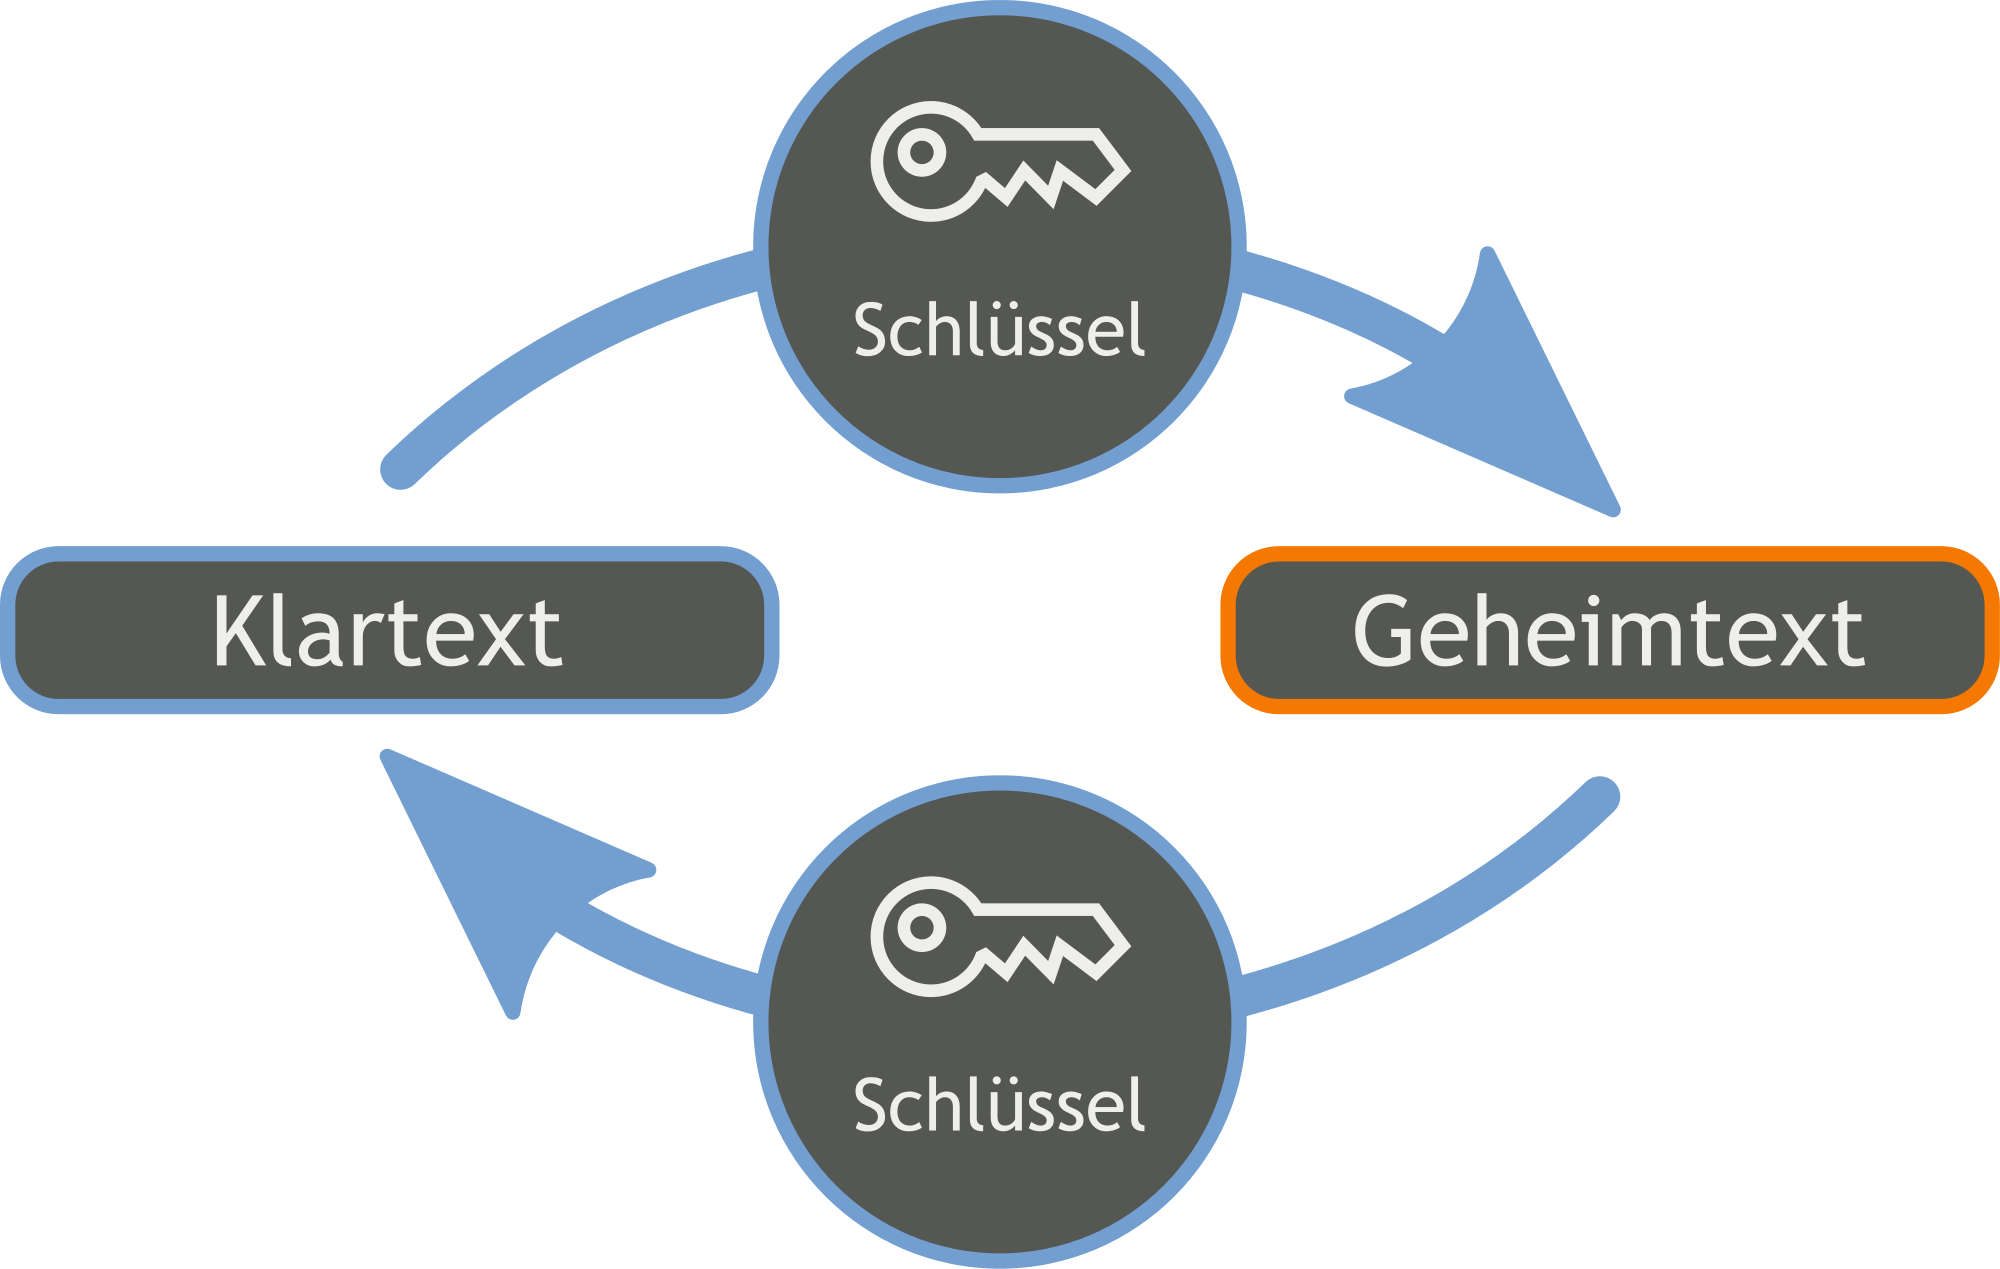
\includegraphics[scale=0.2]{symm_shema.png} %ref link wikipedia
\end{center}

% Daniel
\subsection{Stromchiffren} 
Stromchiffren verarbeiten immer jeden Bit einer Nachricht einzeln, also ein Bit rein ein Bit raus. Dabei kommt es zu dem Problem, dass der Empfänger nicht weiß, an welcher Stelle der Sender im Strom gerade ist und falls mal ein Teil der Nachricht, bei der Übertragung verloren gehen sollte, führt das auch zu Problemen.
\subsection{Blockchiffren}
Blockchiffren verarbeiten immer eine bestimmte Menge an Bits einer Nachricht, in einem ganzen Block. Das Problem, dabei ist, dass manchmal ein Block zu klein ist und somit die Verschlüsselung überhaupt nicht stattfinden kann.

\subsection{Sicherheit}\label{symm:secu}
Die Sicherheit von symmetrsichen Verfahren hängt stark vom Schlüssel ab. Ein zu kurzer Schlüssel zum Beispiel könnte schnell errechnet werden und somit wäre die Kommunitkation nicht mehr Sicher, deshalb ist ein langer Schlüssel\footnote{Heutzutage 1024 Bit.} wichtig, allerdings bringt auch ein langer Schlüssel nichts, wenn er eines Tages an die Öffentlichkeit geraten sollte, denn dann könnte jeder der die Entsprechenden Geheimdaten gesammelt hat den Schlüssel nutzen um diese zu Entschlüsseln. Es ist also sehr wichtig das der Schlüssel geheim bleibt, deshalb ist die Schlüsselverteilung auch ein wichtiger Punkt, wenn man über Sicherheit von symmetrischen Verfahren redet. Die Schlüsselverteilung findet Heutzutage häufig über asymmetrische Verfahren statt oder durch direkten Kontakt der Kommunikationspartner.

\section{Asymetrische Verschlüsselung}\label{asymm}
Asymmetrische Verschlüsselung ist im Vergleich zu symmetrischer noch recht jung. Im Jahr 1975 veröffentlichten Martin Hellman und Whitfield Deffie ihr Deffie-Hellman-Schlusselaustausch Protokoll und damit die ersten Ideen zur asymmetrischen Verschlüsselung. Das erste Wirkliche asymmetrische Verschlüsselungsverfahren wurde allerdings erst 1977 von R. L. Rivest, A. Shamir und L. M. Adleman erfunden. Es erhielt den Namen RSA und ist bis heute immer noch eins der bekanntesten und am häufigsten genutzten Verfahren. Andere bekannte Verfahren sind McEliece(1978), Rabin(1979), Chor-Rivest(1984) und Elgamal(1985).
\subsection{Prinzip asymmetrischer Veschlüsselung}\label{asymm:prinzip}
Asymmetrische Verschlüsselung ist das Gegenstück zu symmetrischer Verschlüsselung, denn hier gibt es nicht nur einen Schlüssel, der für Ver- und Entschlüsselung gebraucht wird, sondern jede Partei einer Kommunikation besitzt einen öffentlichen Schlüssel, welcher für jeden zugänglich ist, und einen privaten Schlüssel, welcher nur der jeweiligen Partei bekannt ist. Wenn jetzt zum Beispiel Partei A einer zweiten Partei B eine Nachricht schicken will, fragt Partei A bei Partei B nach ihrem öffentlichen Schlüssel. Die Übertragung dieses Schlüssels muss nicht sicher sein. Nach dem sie diesen erhalten hat verschlüsselt Partei A ihre Nachricht mit diesem öffentlichen Schlüssel über einen Verschlüsselungsalgrorithmus und erhält einen Geheimtext, den sie selber nicht mehr entschlüsseln kann. Dieser Geheimtext wird dann zu Partei B geschickt und diese kann dann mit hilfe ihres privaten Schlüssels und dem passenden Entschlüsselungsalgorithmus den Geheimtext entschlüsseln. Die Ver- und Entschlüsselungsalgorithmen, welche Partei A und B benutzen, benutzen eine Einwegfunktion mit Falltür(Definition in Kapitel \ref{oneway_trapdoor}), welche als Falltürinformation den jeweiligen privaten Schlüssel benutzt. \newline Folgende Grafik verdeutlicht dieses Schema:
\begin{center}
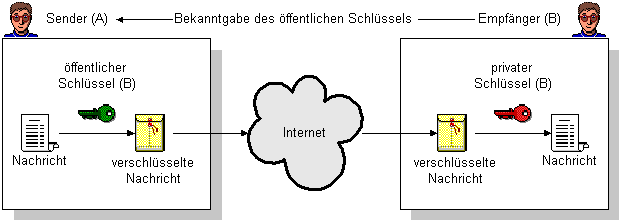
\includegraphics[scale=0.2]{asymm_shema.png} %ref link wikipedia
\end{center}
\subsection{Digitale Signaturen}
Auch wenn das Merkle-Hellman-Kryptosystem keine Signaturen benutzt, sind sie doch ein wichtiger Bestandteil der asymmetrischen Verschlüsselung.
Signaturen werden mithilfe der Einwegfunktion $f(x)$, welche die Ver- /Entschlüsselungsalgorithmen benutzten, erstellt. Die Einwegfunktion muss allerdings eine zusätzliche Eigenschaft haben, sie muss bijektiv sein, das heißt, dass es für jeden $x$ Wert, nur genau einen $y$ Wert gibt und für jeden $y$ Wert, genau einen $x$ Wert.
Wenn jetzt Partei A eine Nachricht $n$ an Partei B schicken will, kehrt Partei A $f(x)$ mit ihrem privaten Schlüssel um und signiert dann mit $f^{-1}(x)$ die Nachricht und erhält die Signatur $s = f^{-1}(m)$. Diese wird dann an Partei B geschickt und die kann dann mit $f(s) = n$ und Partei As öffentlichem Schlüssel, die erhaltene Nachricht verifizieren und weiß nun, dass Partei A die Nachricht geschickt haben muss, da nur sie $f^{-1}(x)$ berechnen konnte.
\subsection{Sicherheit} % Daniel
Asymmetrsiche Verschlüsselungsverfahren haben das Problem der Schlüsselverteilung nicht, weshalb sie gegen über symmetrsichen Verfahren in dem Punkt sicherer sind. Des weiteren gibt es bis jetzt keine effizienten Algorithmen um die beschriebenen Einwegfunktionen umzukehren ohne die entsprechenden Geheiminformationen zu kennen.



\section{Merkle-Hellman Kryptosystem}
Das asymmetrische Merkle-Hellman Kryptosystem wurde 1978 von Ralph Merkle und Martin Hellman erfunden und ist eins der ersten asymmetrischen Kryptosysteme. Es verwendet anders als andere Verfahren(z.B.: RSA) keine digitalen Signaturen. Das Verfahren basiert auf dem Rucksackproblem, welches in Kapitel \ref{rucksack} erläutert wird.

%vergleiche bio merkle & hellman
\subsection{Über die Erfinder}
Ralph Merkle wurde 1952 in Carlifornien geboren. Er schloss 1974 sein Informatikstudium in UC Berkley ab. Im Jahr 1974 stellte er seinen Professoren seine Endeckung zum kryptographischen Schlüsselaustausch, heute bekannt als Merkle's Puzzles, vor. Allerdings hatten sie kein weiteres Interesse an seiner Idee. Doch als er auf Whitfield Diffie und Matrin Hellman traf nam er seine Idee wieder auf und zusammen entwickelten sie Das Merkle-Hellman Kryptosystem. Heutzutage ist Merkle in der Nanotechnologiebranche tätig.  \newline Martin Hellman wurde 1945 in New York geboren. Er schloss sein Studium in Elektrotechnik 1969 an der Standford University ab. Im Jahre 1976 publizierte er zusammen mit Whitfield Diffie einen Artikel über den Deffie-Hellman Schlüsselaustausch und erste Ideen zur asymmetrsichen Verschlüsselung. Heutzutage ist Hellman Professor in Standford im Fach Elektrotechnik.

\subsection{Rucksackproblem}\label{rucksack}
Da das Merkle-Hellman Kryptosystem auf dem Rucksackproblem basiert wird es in diesem Unterkapitel erläutert. \newline Das Rucksackproblem ist leicht mit einem Beispiel zu erklären: Man stelle sich vor man hat einen Rucksack, der nur mit einer bestimmten Menge an Gewicht voll gepackt werden kann. Des weiteren liegen neben dem Rucksack ein paar Gewichte, welche nicht gleich schwer sind und jeweils einen bestimmten Wert haben. Welche Gewichte kommen in den Rucksack so das die Gewichtsgrenze nicht überschritten wird und der maximale Wert(Die Summe aller Werte, der Gewichte im Rucksack) erzielt wird? \newline
Hier ein Beispiel:
\begin{center}
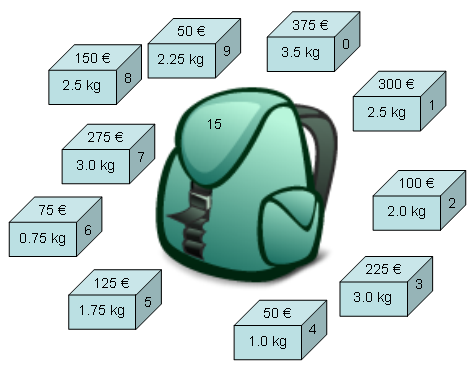
\includegraphics[scale=0.7]{rucksackproblem.png} %ref link wikipedia
\end{center}
Der abgebildete Rucksack kann maximal 15kg tragen. Um ihn herum liegen 10 Gewichte aber welche werden eingepackt? Um dies heraus zu finden werden alle Möglichkeiten, inklusive keine und alle Gewichte im Rucksack, durch probiert und dann geschaut welche Möglichkeiten unter der Gewichtsgrenze liegen und den größten Wert erzielen. Für $n$ Gewichte gibt $2^{n}$ verschiedene Möglichkeiten. Für das Beispiel gibt es also $2^{10} = 1024$ Möglichkeiten. Das sind noch nicht allzu viele und lässt sich deshalb schnell berechnen. Hat man jetzt allerdings weit aus mehr Gewichte lässt sich das Problem nicht mehr effizient lösen. Es gibt eine Ausnahme, welche für das Merkle-Hellman Kryptosystem sehr wichtig ist, diese wird in den nächsten unter Kapiteln erklärt.

%algorithmus
\subsection{Schlüsselerzeugung}
Bei der Schlüsselerzeugung wird zuerst der private Schlüssel generiert, dieser muss ein stark wachsender Vektor seien, dass spielt bei der Entschlüsselung eine entscheidene Rolle, und eine Länge von acht Elementen haben, da ein Buchstabe in Binärcode acht Bits hat. Ein solcher privater Schlüssel $S_p$ könnte folgender Maßen aussehen:
\begin{center}
$S_p=\{44,45,90,180,360,720,1440,2880\}$
\end{center}
Nachdem der private Schlüssel generiert wurde, wird der öffentliche Schlüssel erstellt. Dazu benötigt man zwei weitere Zahlen $m,n$, mit $m,n \in \mathbb{Z}$. $m$ wird so gewählt, dass sie größer ist als die Summe aller Elemente des privaten Schlüssels. Im Fall von $S_p$, mit $k$ als die Anzahl aller Elemente:
\begin{center}
\[m > \sum_{i=0}^{k-1} S_p[i]\]
\end{center}
n wird zufällig gewählt allerdings so, dass der $ggT(m, n) = 1$.
Für unser Beispiel wählen wir $m = 16511$ und $n = 11111$. Um jetzt den öffentlichen Schlüssel $S_{"o}$ zu erstellen, rechnet man für jedes Element $i$:
\begin{center}
\[S_{"o}[i]=(S_p[i] \times n)\; mod \; m\]
\end{center}
Für unseres Beispiel ergibt sich dann der öffentliche Schlüssel:
\begin{center}
$S_{"o}=\{10065,4665,9330,2149,4298,8596,681,1362\}$
\end{center}

\subsection{Verschlüsselung}
Bei der Verschlüsselung wird der Klartext $T_k$ erst in Binärcode umgewandelt. Für das Beispiel wählen wir Hallo als Klartext.
\begin{center}
%$T_k = \{\{0,1,0,0,1,0,0,0\},\{0,1,1,0,0,0,0,1\},\{0,1,1,0,1,1,0,0\},\{0,1,1,0,1,1,0,0\},\{0,1,1,0,1,1,1,1\}\}$
$T_k = \{01101000, 01100001, 01101100, 01101100, 01101111\}$
\end{center} 
Nun wird jeder Bit von jedem Element von $T_k$ mit jedem Element von $S_{"o}$ multipliziert und diese jeweils immer acht Produkte werden addiert, so erhält man die einzelnen ''Geheimbuchstaben'', welche zusammen den Geheimtext $T_g$ ergeben.
Für unser Beispiel:
\begin{center}
$T_g=\{18293,15357,26889,26889,28932\}$
\end{center} 
\subsection{Entschlüsselung}
Zum Entschlüsseln benötigt man $S_p,n,m$ und das modulare Inverse $m^{-1}$ von $m$ und $n$, welches mit dem erweiterten euklidischen Algorithmus berechnet wird.
Für unser Beispiel $m^{-1} = 584$.
Nun wird, um den Klartext zu erhalten, zu erst jedes Element $i$ von $T_g$ mit $m^{-1}$ multipliziert und mit Rest durch m Dividiert.
\begin{center}
\[T_g[i] = (T_g[i] \times m^{-1})\; mod \; m\]
\end{center}
Für das Beispiel ergibt sich die transformierte Version von $T_g$:
\begin{center}
$T_g=\{495,3015,1215,1215,5535\}$
\end{center} 
Danach kommt der Teil in dem die erwähnte Ausnahme des Rucksackproblems wichtig wird. 
Analog stehen hier die Elemente des privaten Schlüssel $S_p$ für die Gewichte, welche alle 1kg wiegen und den Wert $S_p[i]$ haben. Die Gewichtsgrenze des Rucksacks liegt bei 8kg, also würden theoretisch alle Gewichte hinein passen, allerdings wird hier nicht probiert den maximalen Wert zu erreichen, sondern es wird probiert die Werte in $T_g$ zu erreichen und deshalb ist es wichtig das der private Schlüssel ein stark wachsender Vektor ist, denn nur dann ist das Rucksackproblem schnell durch einen Greedyalgorithmus zu lösen. Man erhält als Lösung den Klartext in Binärcodes, in denen eine 1 für ein zutreffendes Element im Schlüssel zur Lösung steht und eine 0 für ein nicht zutreffendes Element. \newline Hier das ganze für den ersten Buchstaben am Beispiel:
\begin{center}
\begin{flushleft}
Für $T_g[0]$ soll eine Lösung aus den Werten von $S_p$ gefunden werden, um den ersten Buchstaben in binär zu erhalten.
\end{flushleft}
\[T_g[0] = 495\]
\begin{flushleft}
Die Lösung lautet $01101000$, da:
\end{flushleft}
\[(0 \times 44) + (1 \times 45) + (1 \times 90) + (0 \times 180) + (1 \times 360)  + (0 \times 720 )+ (0 \times 1440 )+ (0 \times 2880) = 495\]

\begin{flushleft}
Das selbe muss jetzt für jedes Element in $T_g$ getan werden und man erhält den Klartext:
\end{flushleft}

\[T_k = \{01101000, 01100001, 01101100, 01101100, 01101111\}\]

\end{center}

%Für unser Beispiel erhält man dann:
%\begin{center}
%$T_k = \{\}$
%\end{center}
\subsection{Sicherheit}
Zur generellen Sicherheit des Verfahrens sollte man sagen, dass solange $m, n, m^{-1}, S_p$ nicht bekannt sind, es schwer seien sollte das System zu knacken, allerdings hat Adi Shamir, einer der Erfinder des RSA-Vefahrens, es 1982 trotzdem geschafft. Shamirs Methode, zum knacken des Verfahrens ist sehr komplex und würde den Rahmen dieser Facharbeit definitiv sprengen. Des weiteren beinhaltet das Merkle-Hellman-Kryptosystem keine Methoden zum Signieren was mit Hinblick auf die Sicherheit ein großes Problem ist, denn sind zwei Ziele von Verschlüsselung nicht erreicht(Authentizität und Nichtabstreitbarkeit). %merkle-hellman-knapsack-based-public-key-method.pdf



\newpage
\section{Fazit}
\cite{delfs_knebl} \cite{oneway_lukas} \cite{asymm_gesch} \cite{martin_bio} \cite{ralph_bio} \cite{schlusselverteilung} \cite{merklehellman_neer}\cite{fa_asymm_hendrik}
\newpage


%\section{Literaturverzeichnis}
\begin{flushleft}
\bibliography{facharbeit}
\end{flushleft}
%\section{Abbildungsverzeichnis}


\end{document}

